% \renewcommand{\theequation}{\theenumi}
% \begin{enumerate}[label=\arabic*.,ref=\thesubsection.\theenumi]
% \numberwithin{equation}{enumi}

\renewcommand{\theequation}{\theenumi}
\begin{enumerate}[label=\thesection.\arabic*.,ref=\thesection.\theenumi]
\numberwithin{equation}{enumi}


\item How many times must a man toss a fair coin so that the probability of having at least one head is more than 90$\%$?\\
\item An experiment succeeds twice as often as it fails. Find the probability that in the next six trials, there will be at least 4 successes.\\
\solution


As per question,
\begin{align}
    p=2(1-p) \label{eq:2.0.1}\\
    \implies p=2/3\label{eq:2.0.2}
    \end{align}
For a binomial distribution,
\begin {align}
    \pr{X=k}= \comb{n}{k} p^k \brak{1-p}^{n-k}\label{eq:2.0.3}
    \end{align}
For the given question,
\begin{table}[h]
\begin{center}
\begin{tabular}{|c|c|c|}
\hline
 \textbf{Variable} & $n$ & $p$\\
 \hline
 \textbf{Value} & 6 & 2/3\\
 \hline
\end{tabular}
\caption{Value of variables}
\label{Tab 1}
\end{center}
\end{table}
From \eqref{eq:2.0.3} we have,
\begin{align}
\pr{X\geq4}&=\sum_{i=4}^{6}\comb{6}{i} p^i\brak{1-p}^{6-i}
\label{eq: 2.0.4}\\
&=\frac{240}{729}+\frac{192}{729}+\frac{64}{729}
\label{eq: 2.0.5}\\
&=\frac{496}{729}
\label{eq:2.0.6}
\end{align}

\item Suppose X has a binomial distribution . Show that X = 3 is the most likely outcome.\\
\solution
Let X be a binomial random variable which has probability  $p=\frac{1}{2}$ 
 \begin{align}
p(X)=\frac{1}{2} \label{3.3:1}
 \end{align}
Given number of times event(X) is\\
 performed$(n)=6$
 \begin{align}
 n(x)=6 \label{3.3:2}
 \end{align}
Given probability of event$(p)= \frac{1}{2}$\\
Probability that event(X) does not \\occur is
$(1-p)=1-\frac{1}{2}=\frac{1}{2} $
 \begin{align}
1-p(x)=\frac{1}{2}\label{3.3:3}
 \end{align}
We know that binomial probability
\begin{align}
\pr{X=k} = \comb{n}{k} p^k({1-p})^{n-k}  \label{3.3:4} 
\end{align}
For $\pr{X=k}$ to be most likely outcome(highest probability),
 $\pr{X=k}$  should be maximum ,where\\
$ k=\{0,1,2,3,4,5,6\}$\\
To find maximum of  $\pr{X=k}$  ,let us  apply \\logarithm on both sides for equation \eqref{3.3:4} and then diffenrentiate it with respect
to $p$.
\begin{align}
\log  \pr{X=k} &=\log  \comb{n}{k} \times p^k\times ({1-p})^{n-k} \\
&=\log \comb{n}{k} +k \times \log p \notag \\
 &+(n-k)\times log (1-p) \label{3.3:5}
\end{align}
Differentaiate eq \eqref{3.3:5} with respect to p

\begin{align}
\frac{\mathrm{d} \log \pr{X=k} }{\mathrm{d} p}&=\frac{\mathrm{d} \log  \comb{n}{k} }{\mathrm{d}p}+k\times  \frac{\mathrm{d}\log p}{\mathrm{d} p} \\
     &+(n-k) \times \frac{\mathrm{d}\log (1-p)}{\mathrm{d} p} \notag \\
     &=0+\frac{k}{p}-\frac{n-k}{ 1-p} \label{3.3:6}
\end{align}
To find maximum ,substitute $\frac{\mathrm{d} \log  \pr{X=k} }{\mathrm{d} p}=0$ in \eqref{3.3:6}
\begin{align}
\frac{k}{ p}&=\frac{n-k}{1-p}  \\
\frac{ n-k}{k}&=\frac{1-p}{ p}  \\
\frac{ n}{k}-1&=\frac{1}{ p}-1  \\
\frac{n}{ k}&=\frac{ 1}{t p}  \\
k&=n\times p \label{3.3:7}
\end{align}
substituting $n=6,p=1-p=\frac{1}{2}$ in \eqref{3.3:7}\\
We get $k=6\times \frac{1}{2}=3$
$\pr{X=3}$ is maximum,\\
$\therefore\pr{X=3}$ is most likely \\
outcome.\\
(Hint : P(X = 3) is the maximum among all P($x_i$), $x_i$= 0,1,2,3,4,5,6)\\
\item The probability that a bulb produced by a factory will fuse after 150 days of use
is 0.05. Find the probability that out of 5 such bulbs\\
(i) none\\
(ii) not more than one\\
(iii) more than one\\
(iv) at least one\\
will fuse after 150 days of use.\\
\solution
Let X be random variable which denoting number of bulbs fuses after 150 days of use,among the 5 bulbs.Then by Binomial Distribution.
\begin{align}
    \pr{X = r} = {n \choose r} p^r q^{n-r}\\
    \pr{X \geq k} = \sum_{r = k}^n {n \choose r}p^r q^{n-r}\\
    \pr{X \leq k} = \sum_{r = 0}^k {n \choose r}p^r q^{n-r}\\
    \pr{X>k} = \sum_{r=k+1}^{n}{n\choose r}p^r q^{n-r}\\
    n = 5,\quad p = 0.05,\quad q = 0.95
\end{align}

\begin{table}[h!]
\resizebox{\columnwidth}{!}{%
  \begin{tabular}{|c|c|c|c|c|}
    \hline
    n &  5 & 5 & 5& 5\\
    \hline
    Condition & \pr{X = 0} & \pr{X\leq1} & \pr{X > 1} & \pr{X \geq1}\\
    \hline
    Value & 0.77378 & 0.97740 & 0.02259 & 0.22621\\
    \hline
    Case & $(i)$ & $(ii)$ & $(iii)$ & $(iv)$\\
    \hline
  \end{tabular}%
} 
  \caption{ Probability Vs Condition}
  \label{tab:label1_test}
\end{table}  

\item Find the mean number of heads in three tosses of a fair coin.\\
\solution
By observing we can get 4 cases which are 0 heads, 1 heads, 2 heads, 3 heads respectively when 3 fair coins are tossed simultaneously.\\
Let $X_{i}$ be the number of heads in \textit{i}th case .\\
So we can get the probability of number of heads each case  as
\begin{align}
   \pr{X = k} = 
  \begin{cases}
    {^3 C_k}\brak{\frac{1}{2}}^{k}\brak{1-\frac{1}{2}}^{3-k} & 0 \leq k \leq 3\\
    0 & otherwise
  \end{cases}
 \end{align}
 \begin{align}\label{3.5equation-2}
   \pr{X = k} = 
   \begin{cases}
    {^3 C_k}\brak{\frac{1}{2}}^{3} &  0 \leq k \leq 3  \\
    0 & otherwise
  \end{cases}
\end{align}
\\The probability distribution table is \\
\begin{table}[h!]\label{3.5table}
\centering
\begin{tabular}{||c||c||c||c||c||}
\hline\hline
     \textit{i} & 1 & 2 & 3 & 4  \\
     \hline\hline
     $X_{i}$ & 0 & 1 & 2 & 3 \\
     \hline\hline
     $\pr{X = X_{i}}$ & $\frac{1}{8}$ & $\frac{3}{8}$ & $\frac{3}{8}$ & $\frac{1}{8}$\\[1ex]
     \hline\hline
\end{tabular}
\caption{Probability distribution table}
\end{table}
\\Hence by substituing values of \textit{n} = 3 and \textit{p} = $\frac{1}{2}$, we get 
\begin{align}
    E(X) &= np\\
         &= 3 \times \frac{1}{2} \\
         &= \frac{3}{2} \\
         &= 1.5
\end{align}

\item Find the probability distribution of\\
(i) number of heads in two tosses of a coin.\\
(ii) number of tails in the simultaneous tosses of three coins.\\
(iii) number of heads in four tosses of a coin.\\
\solution

\begin{align}\label{3.6:eq1}
   \pr{X=k} =
  \begin{cases*}
    {^n C_k}p^{k}(1-p)^{n-k} & $0 \leq k \leq n$\\
      0 & otherwise
  \end{cases*}
\end{align}

Table \eqref{3.6:Table1} presents the solution to each case.


\begin{table}[h!]
\centering
\caption{Table of Probability distribution of different cases}
\resizebox{.5\textwidth}{!}{
  \begin{tabular}{|c|m{1cm}|m{2cm}|c|c|c|c|c|}
  \hline
    Case &  n (no. of coins) & k (no. of required outcomes) & 0 & 1 & 2 & 3 & 4\\
    \hline
    $(i)$ & 2 & $\pr{X=k}={^2 C_k}\brak{\frac{1}{2}}^{2}$ & $1/2$& $1/4$ & $1/2$ & $0$ & $0$\\
    \hline
    $(ii)$ & 3 & $\pr{X=k}={^3 C_k}\brak{\frac{1}{2}}^{3}$ & $1/8$ & $3/8$ & $3/8$ & $1/8$ & $0$\\
    \hline
    $(iii)$ & 4 & $\pr{X=k}={^4 C_k}\brak{\frac{1}{2}}^{4}$ & $1/16$& $1/4$ & $3/8$ & $1/4$ & $1/16$\\
    \hline
  \end{tabular}
  \label{3.6:Table1}
}
\end{table}

\item Let X represent the difference between the number of heads and the number of tails obtained when a coin is tossed 6 times. What are possible values of X?\\
\item Six balls are drawn successively from an urn containing 7 red and 9 black balls. Tell whether or not the trials of drawing balls are Bernoulli trials when after each draw the ball drawn is\\
(i) replaced \\
(ii) not replaced in the urn.\\
\solution
Properties to be satisfied if a trial needs to be a bernoulli trial:\\
\begin{enumerate}
    \item Number of trials should be finite.
    \item each trial should have utcomes of success and failure.\
    \item if P is the success probability then failure probability should be 1-P
    \item probability of success should not vary with trial
\end{enumerate}

\textbf{Case(i):Replaced} \\ 
Number of red balls = 7\\
Number of black balls = 9\\
let X be the random variable and 
\begin{itemize}
    \item X=1 is success which is Drawing red ball
    \item X=0 is Failure which is Drawing black ball
\end{itemize}
Success Probability 
\begin{equation}
    P(X=1) = \frac{7}{16} 
\end{equation}
Failure Probability
\begin{equation}
     P(X=0) = \frac{9}{16} = 1-P(X=1)
\end{equation}
 Success Probability is  constant for all Trials.
 as X satisfies all properties of Bernoulli therefore Trials are Bernoulli Trials.\\ \\
\textbf{Case(ii):Not Replaced} \\ \\
In this case Success Probability is 
\begin{equation}
    P(X=1) =\frac{7}{16}
\end{equation}
 for Second Trial 
\begin{equation}
     P(X=1) = \frac{6}{15} 
\end{equation} 
 Corresponding Failure Probabilities are 
 \begin{equation}
     P(X=0) = \frac{9}{16}
 \end{equation} and for 2nd trial 
 \begin{equation}
     P(X=0) = \frac{8}{15}
 \end{equation}  
  probability of success and corresponding failure is varying with trials therefore these are not Bernoulli Trials. 
\begin{itemize}
    \item Case(i):Trials are Bernoulli Trials 
    \item Case(ii): Trials are not Bernoulli Trials
\end{itemize}

\item If a fair coin is tossed 10 times, find the probability of
\begin{enumerate}
\item  exactly six heads
\item  at least six heads
\item  at most six  heads
\end{enumerate}
\solution
The given curve 
\begin{align}
	y =\frac{1}{x-1}
\end{align}
can be expressed as 
\begin{align}
	xy - y - 1 = 0 \label{eq:solutions/1/14/eq:hyperbola}
\end{align}
Hence, we have
\begin{align}
	\vec{V} = \frac{1}{2}\myvec{0 & 1 \\ 1 & 0}, 
	\vec{u} = \frac{1}{2}\myvec{0 \\-1},
	f = -1
\end{align}
Since $\mydet{\vec{V}} < 0$, the equation \eqref{eq:solutions/1/14/eq:hyperbola} represents hyperbola.
To find the values of $\lambda_1$ and $\lambda_2$, consider the characteristic equation,
\begin{align}
	\mydet{\lambda\vec{I} - \vec{V}} &= 0\\
	\implies \mydet{\myvec{\lambda & 0\\0 & \lambda} - \myvec{0 & \frac{1}{2} \\ \frac{1}{2} & 0}} &= 0\\
	\implies \mydet{ \lambda & \frac{-1}{2} \\ \frac{-1}{2} & \lambda} &= 0\\
	\implies \lambda_1 &= \frac{1}{2} , \lambda_2 = \frac{-1}{2}
\end{align}
In addition, given the slope -1, the direction and normal vectors are given by 
\begin{align}
	\vec{m} = \myvec{1 \\ -1} \\
	\vec{n} = \myvec{ 1 \\ 1}
\end{align}
The parameters of hyperbola are as follows:
\begin{align}
	\vec{c} &= -\vec{V}^{-1}\vec{u} \\
	&= -\myvec{0 & 2\\ 2 & 0}\myvec{0 \\ -\frac{1}{2}} \\
	&= \myvec{1 \\ 0}\\
	axes &= \begin{cases}
	\sqrt{\frac{\vec{u}^T\vec{V}^{-1}\vec{u} - f}{\lambda_1}} = \sqrt{2}\\
 \sqrt{\frac{f-\vec{u}^T\vec{V}^{-1}\vec{u}}{\lambda_2}} = \sqrt{2}
\end{cases}
\end{align}
which represents the standard hyperbola equation,
\begin{align}
	\frac{x^2}{2} - \frac{x^2}{2} = 1
\end{align}
The points of contact are given by 
\begin{align}
  \tiny{K} &=\pm \sqrt{\frac{\vec{u}^T\vec{V}^{-1}\vec{u} - f}{\vec{n}^T\vec{V}^{-1}\vec{n}}}
  = \pm \frac{1}{2}\\
  \vec{q} &= \vec{V}^{-1}(k\vec{n}-\vec{u})\\
  \vec{q_1} &= \myvec{0 & 2\\2 & 0} \sbrak{\frac{1}{2}\myvec{1 \\ 1} - \myvec{0\\ \frac{-1}{2}}}\\
  &= \myvec{2 \\ 1}\\
  \vec{q_2} &= \myvec{0 & 2\\2 & 0} \sbrak{\frac{-1}{2}\myvec{1 \\ 1} - \myvec{0\\ \frac{-1}{2}}}\\
  &= \myvec{0 \\ -1}
\end{align} 
$\therefore$ The tangents are given by
\begin{align}
	\myvec{1 & 1} \brak{\vec{x} - \myvec{2 \\ 1}} = 0 \\
	\myvec{1 & 1} \brak{\vec{x} - \myvec{0 \\ -1}} = 0
\end{align}
The desired equations of all lines having slope -1 that are tangents to the curve $\frac{1}{x-1}, x \neq 1$ are given by
\begin{align}
	\myvec{1 & 1}\vec{x} &= 3 \\
	\myvec{1 & 1}\vec{x} &= -1 
\end{align}
The above results are verified in the following figure.
\begin{figure}[h!] \label{eq:solutions/1/14/fig:tangents}
	\centering
	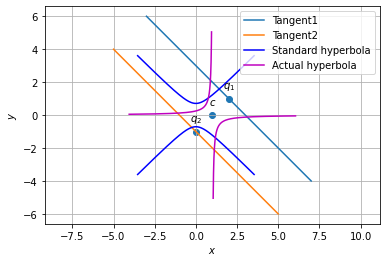
\includegraphics[width=\columnwidth]{./solutions/1/14/graph7.png}
	\caption{The standard and actual hyperbola.}
\end{figure}


\item Ten eggs are drawn successively with replacement from a lot containing 10$\%$ defective eggs. Find the probability that there is at least one defective egg.\\
\solution
The given curve 
\begin{align}
	y =\frac{1}{x-1}
\end{align}
can be expressed as 
\begin{align}
	xy - y - 1 = 0 \label{eq:solutions/1/14/eq:hyperbola}
\end{align}
Hence, we have
\begin{align}
	\vec{V} = \frac{1}{2}\myvec{0 & 1 \\ 1 & 0}, 
	\vec{u} = \frac{1}{2}\myvec{0 \\-1},
	f = -1
\end{align}
Since $\mydet{\vec{V}} < 0$, the equation \eqref{eq:solutions/1/14/eq:hyperbola} represents hyperbola.
To find the values of $\lambda_1$ and $\lambda_2$, consider the characteristic equation,
\begin{align}
	\mydet{\lambda\vec{I} - \vec{V}} &= 0\\
	\implies \mydet{\myvec{\lambda & 0\\0 & \lambda} - \myvec{0 & \frac{1}{2} \\ \frac{1}{2} & 0}} &= 0\\
	\implies \mydet{ \lambda & \frac{-1}{2} \\ \frac{-1}{2} & \lambda} &= 0\\
	\implies \lambda_1 &= \frac{1}{2} , \lambda_2 = \frac{-1}{2}
\end{align}
In addition, given the slope -1, the direction and normal vectors are given by 
\begin{align}
	\vec{m} = \myvec{1 \\ -1} \\
	\vec{n} = \myvec{ 1 \\ 1}
\end{align}
The parameters of hyperbola are as follows:
\begin{align}
	\vec{c} &= -\vec{V}^{-1}\vec{u} \\
	&= -\myvec{0 & 2\\ 2 & 0}\myvec{0 \\ -\frac{1}{2}} \\
	&= \myvec{1 \\ 0}\\
	axes &= \begin{cases}
	\sqrt{\frac{\vec{u}^T\vec{V}^{-1}\vec{u} - f}{\lambda_1}} = \sqrt{2}\\
 \sqrt{\frac{f-\vec{u}^T\vec{V}^{-1}\vec{u}}{\lambda_2}} = \sqrt{2}
\end{cases}
\end{align}
which represents the standard hyperbola equation,
\begin{align}
	\frac{x^2}{2} - \frac{x^2}{2} = 1
\end{align}
The points of contact are given by 
\begin{align}
  \tiny{K} &=\pm \sqrt{\frac{\vec{u}^T\vec{V}^{-1}\vec{u} - f}{\vec{n}^T\vec{V}^{-1}\vec{n}}}
  = \pm \frac{1}{2}\\
  \vec{q} &= \vec{V}^{-1}(k\vec{n}-\vec{u})\\
  \vec{q_1} &= \myvec{0 & 2\\2 & 0} \sbrak{\frac{1}{2}\myvec{1 \\ 1} - \myvec{0\\ \frac{-1}{2}}}\\
  &= \myvec{2 \\ 1}\\
  \vec{q_2} &= \myvec{0 & 2\\2 & 0} \sbrak{\frac{-1}{2}\myvec{1 \\ 1} - \myvec{0\\ \frac{-1}{2}}}\\
  &= \myvec{0 \\ -1}
\end{align} 
$\therefore$ The tangents are given by
\begin{align}
	\myvec{1 & 1} \brak{\vec{x} - \myvec{2 \\ 1}} = 0 \\
	\myvec{1 & 1} \brak{\vec{x} - \myvec{0 \\ -1}} = 0
\end{align}
The desired equations of all lines having slope -1 that are tangents to the curve $\frac{1}{x-1}, x \neq 1$ are given by
\begin{align}
	\myvec{1 & 1}\vec{x} &= 3 \\
	\myvec{1 & 1}\vec{x} &= -1 
\end{align}
The above results are verified in the following figure.
\begin{figure}[h!] \label{eq:solutions/1/14/fig:tangents}
	\centering
	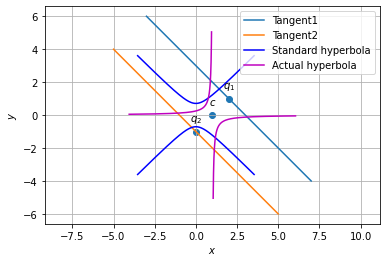
\includegraphics[width=\columnwidth]{./solutions/1/14/graph7.png}
	\caption{The standard and actual hyperbola.}
\end{figure}


\item Find the mean of the Binomial distribution B(4,$\frac{1}{3}$).
\\
\solution
The given curve 
\begin{align}
	y =\frac{1}{x-1}
\end{align}
can be expressed as 
\begin{align}
	xy - y - 1 = 0 \label{eq:solutions/1/14/eq:hyperbola}
\end{align}
Hence, we have
\begin{align}
	\vec{V} = \frac{1}{2}\myvec{0 & 1 \\ 1 & 0}, 
	\vec{u} = \frac{1}{2}\myvec{0 \\-1},
	f = -1
\end{align}
Since $\mydet{\vec{V}} < 0$, the equation \eqref{eq:solutions/1/14/eq:hyperbola} represents hyperbola.
To find the values of $\lambda_1$ and $\lambda_2$, consider the characteristic equation,
\begin{align}
	\mydet{\lambda\vec{I} - \vec{V}} &= 0\\
	\implies \mydet{\myvec{\lambda & 0\\0 & \lambda} - \myvec{0 & \frac{1}{2} \\ \frac{1}{2} & 0}} &= 0\\
	\implies \mydet{ \lambda & \frac{-1}{2} \\ \frac{-1}{2} & \lambda} &= 0\\
	\implies \lambda_1 &= \frac{1}{2} , \lambda_2 = \frac{-1}{2}
\end{align}
In addition, given the slope -1, the direction and normal vectors are given by 
\begin{align}
	\vec{m} = \myvec{1 \\ -1} \\
	\vec{n} = \myvec{ 1 \\ 1}
\end{align}
The parameters of hyperbola are as follows:
\begin{align}
	\vec{c} &= -\vec{V}^{-1}\vec{u} \\
	&= -\myvec{0 & 2\\ 2 & 0}\myvec{0 \\ -\frac{1}{2}} \\
	&= \myvec{1 \\ 0}\\
	axes &= \begin{cases}
	\sqrt{\frac{\vec{u}^T\vec{V}^{-1}\vec{u} - f}{\lambda_1}} = \sqrt{2}\\
 \sqrt{\frac{f-\vec{u}^T\vec{V}^{-1}\vec{u}}{\lambda_2}} = \sqrt{2}
\end{cases}
\end{align}
which represents the standard hyperbola equation,
\begin{align}
	\frac{x^2}{2} - \frac{x^2}{2} = 1
\end{align}
The points of contact are given by 
\begin{align}
  \tiny{K} &=\pm \sqrt{\frac{\vec{u}^T\vec{V}^{-1}\vec{u} - f}{\vec{n}^T\vec{V}^{-1}\vec{n}}}
  = \pm \frac{1}{2}\\
  \vec{q} &= \vec{V}^{-1}(k\vec{n}-\vec{u})\\
  \vec{q_1} &= \myvec{0 & 2\\2 & 0} \sbrak{\frac{1}{2}\myvec{1 \\ 1} - \myvec{0\\ \frac{-1}{2}}}\\
  &= \myvec{2 \\ 1}\\
  \vec{q_2} &= \myvec{0 & 2\\2 & 0} \sbrak{\frac{-1}{2}\myvec{1 \\ 1} - \myvec{0\\ \frac{-1}{2}}}\\
  &= \myvec{0 \\ -1}
\end{align} 
$\therefore$ The tangents are given by
\begin{align}
	\myvec{1 & 1} \brak{\vec{x} - \myvec{2 \\ 1}} = 0 \\
	\myvec{1 & 1} \brak{\vec{x} - \myvec{0 \\ -1}} = 0
\end{align}
The desired equations of all lines having slope -1 that are tangents to the curve $\frac{1}{x-1}, x \neq 1$ are given by
\begin{align}
	\myvec{1 & 1}\vec{x} &= 3 \\
	\myvec{1 & 1}\vec{x} &= -1 
\end{align}
The above results are verified in the following figure.
\begin{figure}[h!] \label{eq:solutions/1/14/fig:tangents}
	\centering
	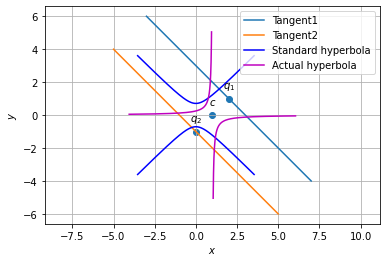
\includegraphics[width=\columnwidth]{./solutions/1/14/graph7.png}
	\caption{The standard and actual hyperbola.}
\end{figure}


\item The probability of a shooter hitting a target is $\frac{3}{4}$. How many minimum
number of times must he/she fire so that the probability of hitting the target at least
once is more than 0.99?
\\
\solution
The given curve 
\begin{align}
	y =\frac{1}{x-1}
\end{align}
can be expressed as 
\begin{align}
	xy - y - 1 = 0 \label{eq:solutions/1/14/eq:hyperbola}
\end{align}
Hence, we have
\begin{align}
	\vec{V} = \frac{1}{2}\myvec{0 & 1 \\ 1 & 0}, 
	\vec{u} = \frac{1}{2}\myvec{0 \\-1},
	f = -1
\end{align}
Since $\mydet{\vec{V}} < 0$, the equation \eqref{eq:solutions/1/14/eq:hyperbola} represents hyperbola.
To find the values of $\lambda_1$ and $\lambda_2$, consider the characteristic equation,
\begin{align}
	\mydet{\lambda\vec{I} - \vec{V}} &= 0\\
	\implies \mydet{\myvec{\lambda & 0\\0 & \lambda} - \myvec{0 & \frac{1}{2} \\ \frac{1}{2} & 0}} &= 0\\
	\implies \mydet{ \lambda & \frac{-1}{2} \\ \frac{-1}{2} & \lambda} &= 0\\
	\implies \lambda_1 &= \frac{1}{2} , \lambda_2 = \frac{-1}{2}
\end{align}
In addition, given the slope -1, the direction and normal vectors are given by 
\begin{align}
	\vec{m} = \myvec{1 \\ -1} \\
	\vec{n} = \myvec{ 1 \\ 1}
\end{align}
The parameters of hyperbola are as follows:
\begin{align}
	\vec{c} &= -\vec{V}^{-1}\vec{u} \\
	&= -\myvec{0 & 2\\ 2 & 0}\myvec{0 \\ -\frac{1}{2}} \\
	&= \myvec{1 \\ 0}\\
	axes &= \begin{cases}
	\sqrt{\frac{\vec{u}^T\vec{V}^{-1}\vec{u} - f}{\lambda_1}} = \sqrt{2}\\
 \sqrt{\frac{f-\vec{u}^T\vec{V}^{-1}\vec{u}}{\lambda_2}} = \sqrt{2}
\end{cases}
\end{align}
which represents the standard hyperbola equation,
\begin{align}
	\frac{x^2}{2} - \frac{x^2}{2} = 1
\end{align}
The points of contact are given by 
\begin{align}
  \tiny{K} &=\pm \sqrt{\frac{\vec{u}^T\vec{V}^{-1}\vec{u} - f}{\vec{n}^T\vec{V}^{-1}\vec{n}}}
  = \pm \frac{1}{2}\\
  \vec{q} &= \vec{V}^{-1}(k\vec{n}-\vec{u})\\
  \vec{q_1} &= \myvec{0 & 2\\2 & 0} \sbrak{\frac{1}{2}\myvec{1 \\ 1} - \myvec{0\\ \frac{-1}{2}}}\\
  &= \myvec{2 \\ 1}\\
  \vec{q_2} &= \myvec{0 & 2\\2 & 0} \sbrak{\frac{-1}{2}\myvec{1 \\ 1} - \myvec{0\\ \frac{-1}{2}}}\\
  &= \myvec{0 \\ -1}
\end{align} 
$\therefore$ The tangents are given by
\begin{align}
	\myvec{1 & 1} \brak{\vec{x} - \myvec{2 \\ 1}} = 0 \\
	\myvec{1 & 1} \brak{\vec{x} - \myvec{0 \\ -1}} = 0
\end{align}
The desired equations of all lines having slope -1 that are tangents to the curve $\frac{1}{x-1}, x \neq 1$ are given by
\begin{align}
	\myvec{1 & 1}\vec{x} &= 3 \\
	\myvec{1 & 1}\vec{x} &= -1 
\end{align}
The above results are verified in the following figure.
\begin{figure}[h!] \label{eq:solutions/1/14/fig:tangents}
	\centering
	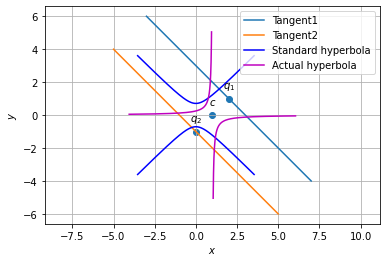
\includegraphics[width=\columnwidth]{./solutions/1/14/graph7.png}
	\caption{The standard and actual hyperbola.}
\end{figure}


\item Three coins are tossed simultaneously. Consider the event E "three heads or three tails", F "at least two heads" and G "at most two heads". Of the pairs (E,F), (E,G) and (F,G), which are independent? which are dependent?\\
\solution
From the given information,
	\begin{align}
	\pr{E} &= \frac{3}{6} = \frac{1}{2} \\
	\pr{F} &= \frac{2}{6} = \frac{1}{3} \\	
	\pr{G} &= \frac{4}{6} = \frac{2}{3} \\	
	\pr{E F} &= \frac{1}{6}\\
	\pr{E G} &= \frac{2}{6}= \frac{1}{3}\\
	\pr{F G} &= \frac{2}{6}= \frac{1}{3}\\
	\pr{E F G} &= \frac{1}{6}
\end{align}
\begin{enumerate}
\item	
\begin{align}
	\pr{E|F} &= \frac{\pr{E F}}{\pr{F}}\\
	\pr{E|F} &= \frac{\frac{1}{6}}{\frac{1}{3}} = \frac{1}{2}\\
	\pr{F|E} &= \frac{\pr{F E}}{\pr{E}}\\
	\pr{F|E} &= \frac{\frac{1}{6}}{\frac{1}{2}} = \frac{1}{3}
	\end{align}

\item 	\begin{align}
	\pr{E|G} &= \frac{\pr{E G}}{\pr{G}}\\
	\pr{E|G} &= \frac{\frac{1}{3}}{\frac{2}{3}} = \frac{1}{2}\\
	\pr{G|E} &= \frac{\pr{G E}}{\pr{G}}\\
	\pr{G|E} &= \frac{\frac{1}{3}}{\frac{1}{2}} = \frac{2}{3}\\
	\end{align}
	
\item	%$\pr{\frac{E\cup F}{G}}$
\begin{multline}
\pr{E+F|G} = \frac{\pr{\cbrak{E+F}G}}{\pr{G}}
\\
 = \frac{\pr{EG + FG}}{\pr{G}}
\\
=\frac{\pr{EG} +\pr{ FG}- \pr{EFG}}{\pr{G}}
\\
 = \frac{3}{4}
\end{multline}
and 
\begin{align}
\pr{EF|G} = 
\frac{ \pr{EFG}}{\pr{G}}
 = \frac{1}{4}
\end{align}

\end{enumerate}

\item A die is tossed thrice. Find the probability of getting an odd number at least once.\\
\\
\solution
The given curve 
\begin{align}
	y =\frac{1}{x-1}
\end{align}
can be expressed as 
\begin{align}
	xy - y - 1 = 0 \label{eq:solutions/1/14/eq:hyperbola}
\end{align}
Hence, we have
\begin{align}
	\vec{V} = \frac{1}{2}\myvec{0 & 1 \\ 1 & 0}, 
	\vec{u} = \frac{1}{2}\myvec{0 \\-1},
	f = -1
\end{align}
Since $\mydet{\vec{V}} < 0$, the equation \eqref{eq:solutions/1/14/eq:hyperbola} represents hyperbola.
To find the values of $\lambda_1$ and $\lambda_2$, consider the characteristic equation,
\begin{align}
	\mydet{\lambda\vec{I} - \vec{V}} &= 0\\
	\implies \mydet{\myvec{\lambda & 0\\0 & \lambda} - \myvec{0 & \frac{1}{2} \\ \frac{1}{2} & 0}} &= 0\\
	\implies \mydet{ \lambda & \frac{-1}{2} \\ \frac{-1}{2} & \lambda} &= 0\\
	\implies \lambda_1 &= \frac{1}{2} , \lambda_2 = \frac{-1}{2}
\end{align}
In addition, given the slope -1, the direction and normal vectors are given by 
\begin{align}
	\vec{m} = \myvec{1 \\ -1} \\
	\vec{n} = \myvec{ 1 \\ 1}
\end{align}
The parameters of hyperbola are as follows:
\begin{align}
	\vec{c} &= -\vec{V}^{-1}\vec{u} \\
	&= -\myvec{0 & 2\\ 2 & 0}\myvec{0 \\ -\frac{1}{2}} \\
	&= \myvec{1 \\ 0}\\
	axes &= \begin{cases}
	\sqrt{\frac{\vec{u}^T\vec{V}^{-1}\vec{u} - f}{\lambda_1}} = \sqrt{2}\\
 \sqrt{\frac{f-\vec{u}^T\vec{V}^{-1}\vec{u}}{\lambda_2}} = \sqrt{2}
\end{cases}
\end{align}
which represents the standard hyperbola equation,
\begin{align}
	\frac{x^2}{2} - \frac{x^2}{2} = 1
\end{align}
The points of contact are given by 
\begin{align}
  \tiny{K} &=\pm \sqrt{\frac{\vec{u}^T\vec{V}^{-1}\vec{u} - f}{\vec{n}^T\vec{V}^{-1}\vec{n}}}
  = \pm \frac{1}{2}\\
  \vec{q} &= \vec{V}^{-1}(k\vec{n}-\vec{u})\\
  \vec{q_1} &= \myvec{0 & 2\\2 & 0} \sbrak{\frac{1}{2}\myvec{1 \\ 1} - \myvec{0\\ \frac{-1}{2}}}\\
  &= \myvec{2 \\ 1}\\
  \vec{q_2} &= \myvec{0 & 2\\2 & 0} \sbrak{\frac{-1}{2}\myvec{1 \\ 1} - \myvec{0\\ \frac{-1}{2}}}\\
  &= \myvec{0 \\ -1}
\end{align} 
$\therefore$ The tangents are given by
\begin{align}
	\myvec{1 & 1} \brak{\vec{x} - \myvec{2 \\ 1}} = 0 \\
	\myvec{1 & 1} \brak{\vec{x} - \myvec{0 \\ -1}} = 0
\end{align}
The desired equations of all lines having slope -1 that are tangents to the curve $\frac{1}{x-1}, x \neq 1$ are given by
\begin{align}
	\myvec{1 & 1}\vec{x} &= 3 \\
	\myvec{1 & 1}\vec{x} &= -1 
\end{align}
The above results are verified in the following figure.
\begin{figure}[h!] \label{eq:solutions/1/14/fig:tangents}
	\centering
	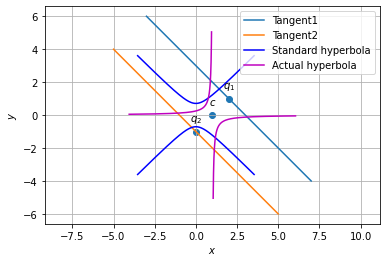
\includegraphics[width=\columnwidth]{./solutions/1/14/graph7.png}
	\caption{The standard and actual hyperbola.}
\end{figure}

\item A game consists of tossing a one rupee coin 3 times and noting its outcome each time. Hanif wins if all the tosses give the same result i.e., three heads or three tails, and loses otherwise. Calculate the probability that Hanif will lose the game.
\\
\solution
The given curve 
\begin{align}
	y =\frac{1}{x-1}
\end{align}
can be expressed as 
\begin{align}
	xy - y - 1 = 0 \label{eq:solutions/1/14/eq:hyperbola}
\end{align}
Hence, we have
\begin{align}
	\vec{V} = \frac{1}{2}\myvec{0 & 1 \\ 1 & 0}, 
	\vec{u} = \frac{1}{2}\myvec{0 \\-1},
	f = -1
\end{align}
Since $\mydet{\vec{V}} < 0$, the equation \eqref{eq:solutions/1/14/eq:hyperbola} represents hyperbola.
To find the values of $\lambda_1$ and $\lambda_2$, consider the characteristic equation,
\begin{align}
	\mydet{\lambda\vec{I} - \vec{V}} &= 0\\
	\implies \mydet{\myvec{\lambda & 0\\0 & \lambda} - \myvec{0 & \frac{1}{2} \\ \frac{1}{2} & 0}} &= 0\\
	\implies \mydet{ \lambda & \frac{-1}{2} \\ \frac{-1}{2} & \lambda} &= 0\\
	\implies \lambda_1 &= \frac{1}{2} , \lambda_2 = \frac{-1}{2}
\end{align}
In addition, given the slope -1, the direction and normal vectors are given by 
\begin{align}
	\vec{m} = \myvec{1 \\ -1} \\
	\vec{n} = \myvec{ 1 \\ 1}
\end{align}
The parameters of hyperbola are as follows:
\begin{align}
	\vec{c} &= -\vec{V}^{-1}\vec{u} \\
	&= -\myvec{0 & 2\\ 2 & 0}\myvec{0 \\ -\frac{1}{2}} \\
	&= \myvec{1 \\ 0}\\
	axes &= \begin{cases}
	\sqrt{\frac{\vec{u}^T\vec{V}^{-1}\vec{u} - f}{\lambda_1}} = \sqrt{2}\\
 \sqrt{\frac{f-\vec{u}^T\vec{V}^{-1}\vec{u}}{\lambda_2}} = \sqrt{2}
\end{cases}
\end{align}
which represents the standard hyperbola equation,
\begin{align}
	\frac{x^2}{2} - \frac{x^2}{2} = 1
\end{align}
The points of contact are given by 
\begin{align}
  \tiny{K} &=\pm \sqrt{\frac{\vec{u}^T\vec{V}^{-1}\vec{u} - f}{\vec{n}^T\vec{V}^{-1}\vec{n}}}
  = \pm \frac{1}{2}\\
  \vec{q} &= \vec{V}^{-1}(k\vec{n}-\vec{u})\\
  \vec{q_1} &= \myvec{0 & 2\\2 & 0} \sbrak{\frac{1}{2}\myvec{1 \\ 1} - \myvec{0\\ \frac{-1}{2}}}\\
  &= \myvec{2 \\ 1}\\
  \vec{q_2} &= \myvec{0 & 2\\2 & 0} \sbrak{\frac{-1}{2}\myvec{1 \\ 1} - \myvec{0\\ \frac{-1}{2}}}\\
  &= \myvec{0 \\ -1}
\end{align} 
$\therefore$ The tangents are given by
\begin{align}
	\myvec{1 & 1} \brak{\vec{x} - \myvec{2 \\ 1}} = 0 \\
	\myvec{1 & 1} \brak{\vec{x} - \myvec{0 \\ -1}} = 0
\end{align}
The desired equations of all lines having slope -1 that are tangents to the curve $\frac{1}{x-1}, x \neq 1$ are given by
\begin{align}
	\myvec{1 & 1}\vec{x} &= 3 \\
	\myvec{1 & 1}\vec{x} &= -1 
\end{align}
The above results are verified in the following figure.
\begin{figure}[h!] \label{eq:solutions/1/14/fig:tangents}
	\centering
	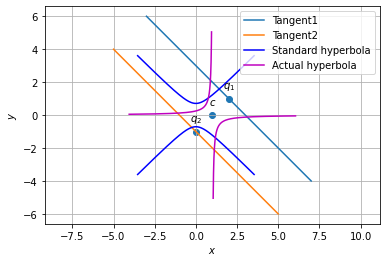
\includegraphics[width=\columnwidth]{./solutions/1/14/graph7.png}
	\caption{The standard and actual hyperbola.}
\end{figure}

\item A die is thrown twice. What is the probability that\\
\begin{enumerate}[label=(\roman*)]
\item  5 will not come up either time? \\
\item  5 will come up at least once?\\
\end{enumerate}
Hint : Throwing a die twice and throwing two dice simultaneously are treated as the
same experiment
\\
\solution
The given curve 
\begin{align}
	y =\frac{1}{x-1}
\end{align}
can be expressed as 
\begin{align}
	xy - y - 1 = 0 \label{eq:solutions/1/14/eq:hyperbola}
\end{align}
Hence, we have
\begin{align}
	\vec{V} = \frac{1}{2}\myvec{0 & 1 \\ 1 & 0}, 
	\vec{u} = \frac{1}{2}\myvec{0 \\-1},
	f = -1
\end{align}
Since $\mydet{\vec{V}} < 0$, the equation \eqref{eq:solutions/1/14/eq:hyperbola} represents hyperbola.
To find the values of $\lambda_1$ and $\lambda_2$, consider the characteristic equation,
\begin{align}
	\mydet{\lambda\vec{I} - \vec{V}} &= 0\\
	\implies \mydet{\myvec{\lambda & 0\\0 & \lambda} - \myvec{0 & \frac{1}{2} \\ \frac{1}{2} & 0}} &= 0\\
	\implies \mydet{ \lambda & \frac{-1}{2} \\ \frac{-1}{2} & \lambda} &= 0\\
	\implies \lambda_1 &= \frac{1}{2} , \lambda_2 = \frac{-1}{2}
\end{align}
In addition, given the slope -1, the direction and normal vectors are given by 
\begin{align}
	\vec{m} = \myvec{1 \\ -1} \\
	\vec{n} = \myvec{ 1 \\ 1}
\end{align}
The parameters of hyperbola are as follows:
\begin{align}
	\vec{c} &= -\vec{V}^{-1}\vec{u} \\
	&= -\myvec{0 & 2\\ 2 & 0}\myvec{0 \\ -\frac{1}{2}} \\
	&= \myvec{1 \\ 0}\\
	axes &= \begin{cases}
	\sqrt{\frac{\vec{u}^T\vec{V}^{-1}\vec{u} - f}{\lambda_1}} = \sqrt{2}\\
 \sqrt{\frac{f-\vec{u}^T\vec{V}^{-1}\vec{u}}{\lambda_2}} = \sqrt{2}
\end{cases}
\end{align}
which represents the standard hyperbola equation,
\begin{align}
	\frac{x^2}{2} - \frac{x^2}{2} = 1
\end{align}
The points of contact are given by 
\begin{align}
  \tiny{K} &=\pm \sqrt{\frac{\vec{u}^T\vec{V}^{-1}\vec{u} - f}{\vec{n}^T\vec{V}^{-1}\vec{n}}}
  = \pm \frac{1}{2}\\
  \vec{q} &= \vec{V}^{-1}(k\vec{n}-\vec{u})\\
  \vec{q_1} &= \myvec{0 & 2\\2 & 0} \sbrak{\frac{1}{2}\myvec{1 \\ 1} - \myvec{0\\ \frac{-1}{2}}}\\
  &= \myvec{2 \\ 1}\\
  \vec{q_2} &= \myvec{0 & 2\\2 & 0} \sbrak{\frac{-1}{2}\myvec{1 \\ 1} - \myvec{0\\ \frac{-1}{2}}}\\
  &= \myvec{0 \\ -1}
\end{align} 
$\therefore$ The tangents are given by
\begin{align}
	\myvec{1 & 1} \brak{\vec{x} - \myvec{2 \\ 1}} = 0 \\
	\myvec{1 & 1} \brak{\vec{x} - \myvec{0 \\ -1}} = 0
\end{align}
The desired equations of all lines having slope -1 that are tangents to the curve $\frac{1}{x-1}, x \neq 1$ are given by
\begin{align}
	\myvec{1 & 1}\vec{x} &= 3 \\
	\myvec{1 & 1}\vec{x} &= -1 
\end{align}
The above results are verified in the following figure.
\begin{figure}[h!] \label{eq:solutions/1/14/fig:tangents}
	\centering
	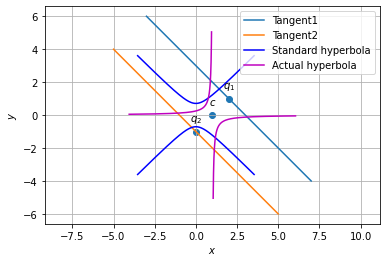
\includegraphics[width=\columnwidth]{./solutions/1/14/graph7.png}
	\caption{The standard and actual hyperbola.}
\end{figure}

\item A die is thrown again and again until three sixes are obtained. Find the probability of obtaining the third six in the sixth throw of the die.\\
\solution
For the 3rd six to occur in the 6th trial, 2 sixes should compulsorily occur in 5 trials.  Defining $X \sim B\brak{5,\frac{1}{6}}$, this probability is given by
\begin{align}
\pr{X = 2} = \comb{5}{2}\brak{\frac{1}{6}}^2\brak{\frac{5}{6}}^3
\end{align}
%
The desired probability is then obtained as
\begin{align}
    \pr{X=2}\times\frac{1}{6} = \frac{625}{23328} 
\end{align}

%
\item Find the probability of throwing at most 2 sixes in 6 throws of a single die.\\
\solution
Defining $X \sim B\brak{6,\frac{1}{5}}$, the desired probability is given by

\begin{align}
\pr{X \leq 2} &=  \sum_{k=0}^{2} \comb{6}{k}\brak{\frac{1}{6}}^k\brak{\frac{5}{6}}^{6-k} \\
&= \brak{\frac{5}{6}}^4 \times \frac{35}{18}\\
&= 0.9377
\end{align}
%
\item In a box containing 100 bulbs, 10 are defective. The probability that out of a
sample of 5 bulbs, none is defective is
\begin{enumerate}
\item $10^{-1}$
\item $\brak{\frac{1}{2}}^5$
\item $\brak{\frac{9}{10}}^5$
\item $\frac{9}{10}$
\end{enumerate}
%
\solution
From the given information, the probability of a bulb being defective is
\begin{align}
p = \frac{10}{100} = \frac{1}{10}
\end{align}
%
Defining $X \sim B \brak{5,\frac{1}{10}}$  the desired probability is
\begin{align}
    \pr{X=0} &= \comb{5}{0} \brak{\frac{1}{10}}^{0} \brak{\frac{9}{10}} ^ {5-0}\\
    &= \brak{\frac{9}{10}}^5
\end{align}

\item In a hurdle race, a player has to cross 10 hurdles. The probability that he will
clear each hurdle is $\frac{5}{6}$. What is the probability that he will knock down fewer than 2 hurdles?\\
\solution 
The given curve 
\begin{align}
	y =\frac{1}{x-1}
\end{align}
can be expressed as 
\begin{align}
	xy - y - 1 = 0 \label{eq:solutions/1/14/eq:hyperbola}
\end{align}
Hence, we have
\begin{align}
	\vec{V} = \frac{1}{2}\myvec{0 & 1 \\ 1 & 0}, 
	\vec{u} = \frac{1}{2}\myvec{0 \\-1},
	f = -1
\end{align}
Since $\mydet{\vec{V}} < 0$, the equation \eqref{eq:solutions/1/14/eq:hyperbola} represents hyperbola.
To find the values of $\lambda_1$ and $\lambda_2$, consider the characteristic equation,
\begin{align}
	\mydet{\lambda\vec{I} - \vec{V}} &= 0\\
	\implies \mydet{\myvec{\lambda & 0\\0 & \lambda} - \myvec{0 & \frac{1}{2} \\ \frac{1}{2} & 0}} &= 0\\
	\implies \mydet{ \lambda & \frac{-1}{2} \\ \frac{-1}{2} & \lambda} &= 0\\
	\implies \lambda_1 &= \frac{1}{2} , \lambda_2 = \frac{-1}{2}
\end{align}
In addition, given the slope -1, the direction and normal vectors are given by 
\begin{align}
	\vec{m} = \myvec{1 \\ -1} \\
	\vec{n} = \myvec{ 1 \\ 1}
\end{align}
The parameters of hyperbola are as follows:
\begin{align}
	\vec{c} &= -\vec{V}^{-1}\vec{u} \\
	&= -\myvec{0 & 2\\ 2 & 0}\myvec{0 \\ -\frac{1}{2}} \\
	&= \myvec{1 \\ 0}\\
	axes &= \begin{cases}
	\sqrt{\frac{\vec{u}^T\vec{V}^{-1}\vec{u} - f}{\lambda_1}} = \sqrt{2}\\
 \sqrt{\frac{f-\vec{u}^T\vec{V}^{-1}\vec{u}}{\lambda_2}} = \sqrt{2}
\end{cases}
\end{align}
which represents the standard hyperbola equation,
\begin{align}
	\frac{x^2}{2} - \frac{x^2}{2} = 1
\end{align}
The points of contact are given by 
\begin{align}
  \tiny{K} &=\pm \sqrt{\frac{\vec{u}^T\vec{V}^{-1}\vec{u} - f}{\vec{n}^T\vec{V}^{-1}\vec{n}}}
  = \pm \frac{1}{2}\\
  \vec{q} &= \vec{V}^{-1}(k\vec{n}-\vec{u})\\
  \vec{q_1} &= \myvec{0 & 2\\2 & 0} \sbrak{\frac{1}{2}\myvec{1 \\ 1} - \myvec{0\\ \frac{-1}{2}}}\\
  &= \myvec{2 \\ 1}\\
  \vec{q_2} &= \myvec{0 & 2\\2 & 0} \sbrak{\frac{-1}{2}\myvec{1 \\ 1} - \myvec{0\\ \frac{-1}{2}}}\\
  &= \myvec{0 \\ -1}
\end{align} 
$\therefore$ The tangents are given by
\begin{align}
	\myvec{1 & 1} \brak{\vec{x} - \myvec{2 \\ 1}} = 0 \\
	\myvec{1 & 1} \brak{\vec{x} - \myvec{0 \\ -1}} = 0
\end{align}
The desired equations of all lines having slope -1 that are tangents to the curve $\frac{1}{x-1}, x \neq 1$ are given by
\begin{align}
	\myvec{1 & 1}\vec{x} &= 3 \\
	\myvec{1 & 1}\vec{x} &= -1 
\end{align}
The above results are verified in the following figure.
\begin{figure}[h!] \label{eq:solutions/1/14/fig:tangents}
	\centering
	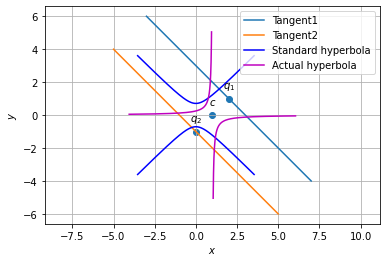
\includegraphics[width=\columnwidth]{./solutions/1/14/graph7.png}
	\caption{The standard and actual hyperbola.}
\end{figure}

\item Suppose that 90$\%$ of people are right-handed. What is the probability that
at most 6 of a random sample of 10 people are right-handed?\\
\solution
From the given information, the random variable in question is $X \sim B\brak{10,\frac{9}{10}}$.
The desired probability is then given by 
\begin{align}
\pr{X\le 6} & = 1-P(X>6) \\ 
              &  =1-\sum_{k=7}^{10}\comb{10}{k}\brak{\frac{9}{10}}^k\brak{\frac{1}{10}}^{10-k} \\
             &=1-\frac{9^7\times 2064}{10^{10}}\\ 
             &=.0128
\end{align}            
\item The probability that a student is not a swimmer is $\frac{1}{5}$. Then the probability that out of five students, four are swimmers is\\
\begin{enumerate}
\item $\comb{5}{4}\brak{\frac{4}{5}}^4 \frac{1}{5}$
\item $\brak{\frac{4}{5}}^4 \frac{1}{5}$
\item $\comb{5}{1}\brak{\frac{4}{5}}^4 \frac{1}{5}$
\item None of these
\end{enumerate}
\solution
Let X be the number of swimmers and the probability that student is swimmer is
\begin{align}
p=\frac{4}{5}
\end{align}
%
Then the desired probability is
\begin{align}
\pr{X=4}=\comb{5}{4}\brak{\frac{4}{5}}^4\brak{\frac{1}{5}}
\end{align}

%
\item A die is thrown 6 times. If ‘getting an odd number’ is a success, what is the probability of\\
(i) 5 successes?\\
(ii) at least 5 successes?\\
(iii) at most 5 successes?\\
%
\solution
let $X \sim B\brak{5,\frac{1}{2}}$ denote the random variable in question.  Then
\begin{enumerate}
\item 
\begin{align}
\pr{X=5} &= \comb{6}{5}\brak{\frac{1}{2}}^5\brak{\frac{1}{2}}^{6-5}
\\
&=\frac{3}{32}
\end{align}
\item 
\begin{align}
\pr{X \ge 5} &= \sum_{k=5}^{6}\comb{6}{5}\brak{\frac{1}{2}}^k\brak{\frac{1}{2}}^{6-k}
\\
&= 0.109375
\end{align}
\item 
\begin{align}
\pr{X \le 5} &= 1 - \pr{X = 6}
\\
&=1-\comb{6}{6}\brak{\frac{1}{2}}^6\brak{\frac{1}{2}}^{6-6}
\\
&= \frac{63}{64}
\end{align}

\end{enumerate}


\item A bag consists of 10 balls each marked with one of the digits 0 to 9. If four balls are drawn successively with replacement from the bag, what is the probability that none is marked with the digit 0?\\
\solution
Let $X$ be number marked on ball drawn.
Since the balls are drawn with replacement, the trials are Bernoulli trials.
\\
So $X$ has Binomial Distribution 
\begin{equation}
    \pr {X=k}=\comb{n}{k} \times q^{n-k} \times p^{k} 
\end{equation} 

Here,
\begin{align}
& n = \text {number of times we pick the ball}  \\
& p= \text{Probability of getting ball marked as 0} \\
& q=1-p
\end{align}

\begin{table}[h!]
\centering

\begin{tabular}{|c|c|c|c|c|}
\hline
\textbf{Variables} & $n$ & $p$    & $q$    & $k$          \\ \hline
\textbf{Values}    & 4 & 1/10 & 9/10 & 0 \\ \hline
\end{tabular}
\caption{Variables and their values}
\label{4.7:table:1}
\end{table}

Now,

\begin{align}
\pr{X=0} &= \comb{4}{0} \times \brak{\frac{9}{10}}^{(4-0)} \times \brak{\frac{1}{10}}^{0} \\
&=\frac{4!}{(4-0)! 0!} \times 1 \times \brak{\frac{9}{10}}^{4} \\
&=\brak { \frac{9}{10} } ^{4} \\
&= 0.6561
\end{align}
%
\item An urn contains 25 balls of which 10 balls bear a mark 'X' and the remaining 15 bear a mark 'Y'. A ball is drawn at random from the urn, its mark is noted down and it is replaced. If 6 balls are drawn in this way, find the probability that\\
(i) all will bear 'X' mark.\\
(ii) not more than 2 will bear 'Y' mark.\\
(iii) at least one ball will bear 'Y' mark.\\
(iv) the number of balls with 'X' mark and 'Y' mark will be equal.\\
\solution
Let X be the number of balls which have 'X' mark on them\\
Using the expression of binomial distribution
\begin{align}
    P(X = r) = {n \choose r} p^r q^{n-r}\\
    P(X \geq k) = \sum_{r = k}^n {n \choose r}p^r q^{n-r}\\
    P(X \leq k) = \sum_{r = 0}^k {n \choose r}p^r q^{n-r}\\
    n = 6,\quad p = 0.4,\quad q = 0.6
\end{align}
\begin{table}[]
\resizebox{\columnwidth}{!}{
    \begin{tabular}{|c|c|c|c|c|}
        \hline
        n & 6 & 6 & 6 & 6\\
        \hline
        Condition & $P(X = 6)$& $P(X \geq 4)$& $P(X \leq 5)$ & $P(X = 3)$ \\
        \hline
        Value & 0.004096 & 0.1792 & 0.995904 & 0.27648\\
        \hline
        Case & $(i)$ & $(ii)$ & $(iii)$ & $(iv)$\\
        \hline
    \end{tabular}
}
\caption{Probabilities of each case }    \label{tab:my_label}
\end{table}


\item It is known that 10$\%$ of certain articles manufactured are defective. What is the probability that in a random sample of 12 such articles, 9 are defective?\\
\solution $X = B \brak{n,p}$ with $n=12$ and $p=\frac{1}{10}$.  Hence, the desired probability is
%
\begin{align}
  \implies\Pr\brak{X=9} &={12 \choose 9}\times\brak{\frac{1}{10}}^9\times\brak{\frac{9}{10}}^{3} \\  &=\frac{16038}{10^{11}}
\end{align}
\item On a multiple choice examination with three possible answers for each of the five questions, what is the probability that a candidate would get four or more correct answers just by guessing ?
\\
\solution
Let $X_i \in (0,1)$ be a random variable where $X_i=1$ represents a successful guess and $X_i = 0$ represents unsuccessful guess on the $i^{th}$ question.\\
\begin{align}
 p=\frac{1}{3}  \notag \\
X= \sum_{i=1}^{n}X_{i} 
\end{align}

where n is the total number of questions. So, X has a binomial distribution.\\
\begin{align}
\pr{X \geq r} = \sum_{k=r}^{n} \binom{n}{r}p^k(1-p)^{n-k} \label{1.0.2} 
\end{align}

Now, in this case n=5 and r=4. From \eqref{1.0.2}\\
\begin{align}
\pr{X=4}=\frac{10}{243}  \notag \\ 
 \pr{X=5}=\frac{1}{243}   \notag \\ 
 \notag
 \end{align}
Hence, required probability= $\frac{11}{243}$ 

\item Five cards are drawn successively with replacement from a well shuffled deck of 52 cards. What is the probability that\\
(i) all the five cards are spades?\\
(ii) only 3 cards are spades?\\
(iii) none is a spade?\\
\solution 
Let $X_{i} \in (0,1)$ be a random variable which denotes whether spade is drawn at the $i^{th}$ draw.\\
   \begin{align}  
      X=\sum_{i=1}^{i=5}X_{i} 
      \end{align}
     where X denotes the number of spades obtained. \\
    \begin{align}
     Since, \pr{x}=\frac{ \text{number of favourable outcome}}{\text{total number of outcomes}} \notag \\
      \pr{x}=\frac{\comb{13}{x}\times \comb{39}{5-x}}{\comb{52}{5}} \label{5.8-1:2.0.2}
      \end{align}
      

\begin{table}[h]
\resizebox{\columnwidth}{!}{
    \begin{tabular}{|l|l|l|l|l|l|l|}
        \hline
        X    & 0 & 1 & 2  & 3  & 4  & 5                     \\ \hline 

P(X) & $\frac{\comb{13}{0}\times\comb{39}{5}}{\comb{52}{5}}$ & $\frac{\comb{13}{1}\times\comb{39}{4}}{\comb{52}{5}}$ & $\frac{\comb{13}{2}\times\comb{39}{3}}{\comb{52}{5}}$ & $\frac{\comb{13}{3}\times\comb{39}{2}}{\comb{52}{5}}$ & $\frac{\comb{13}{4}\times\comb{39}{1}}{\comb{52}{5}}$ & $\frac{\comb{13}{5}\times\comb{39}{0}}{\comb{52}{5}}$ \\ 
\hline

    \end{tabular}
}
\caption{Probabilities of each case }    \label{5.8-1:tab:my_label}
\end{table}

\item Two dice are thrown simultaneously. If X denotes the number of sixes, find the
expectation of X.\\
\solution
Two dice are thrown simultaneously. If $X$ denotes the number of sixes, find the
expectation of $X$
\section*{SOLUTION :}
 When 2 fair dice are thrown simultaneously we know that each die has 6 possible 
 outcomes and outcome of one dice is independent of the outcome of other dice.
 \\$\therefore$ Total possible outcomes are $^{6}C_{1}\,\times\,^{6}C_{1}=36$
 \null \par \null
Let X be a random variable denoting number of sixes in the above case. Then by Binomial
Distribution 
\begin{align}
    \pr{X=k}&=\binom{n}{k}\,p^k\,\brak{1-p}^{n-k} \label{a} \\
    k&=0,\dots,n \label{b}
\end{align}
\begin{align}
\text{Where}\;k &= 0,1,2\\
              n &= 2 \\
              p &= \text{Probability of outcome 6 on a dice} \\
              p &= \dfrac{1}{6}
\end{align}
\null \par \null
From equation \eqref{a} we obtain the following
\newpage
\begin{align}
\pr{X=0} &= \binom{2}{0}\,\brak{\dfrac{1}{6}}^{0}\,\brak{1-\dfrac{1}{6}}^{2} =\dfrac{25}{36} \\
\pr{X=1} &= \binom{2}{1}\,\brak{\dfrac{1}{6}}^{1}\,\brak{1-\dfrac{1}{6}}^{1} =\dfrac{10}{36} \\
\pr{X=2} &= \binom{2}{2}\,\brak{\dfrac{1}{6}}^{2}\,\brak{1-\dfrac{1}{6}}^{0} =\dfrac{1}{36} \\
\end{align}
The probability distribution table is 
\begin{table}[hbt!]
\begin{tabular}{|l|c|c|c|}
\hline
\multicolumn{1}{|c|}{X} & 0 & 1 & 2 \\ \hline
\pr{X=k}                    &$\dfrac{25}{36}$   &$\dfrac{10}{36}$   &$\dfrac{1}{36}$ \\ \hline
\end{tabular}
\end{table}
\begin{align}
\mathbb{E}(X=k) & =\sum_{k=0}^{n} k\pr{k}\\
    & =\sum_{k=0}^{n} k\,\binom{n}{k}\,p^k\,\brak{1-p}^{n-k}\\ 
    & = n\cdot p\,\sum_{k=1}^{n-1} \binom{n-1}{k-1}\,p^{k-1}\,\brak{1-p}^{(n-1)-(k-1)}\\
    & = n\cdot p\,\brak{1 + (1-p)}^{n-1}\\
    & = n \cdot p \\
 \mathbb{E}(X=k) &= n\cdot p = 2\times\dfrac{1}{6} = \dfrac{1}{3}
\end{align}

\\
\item Find the variance of the number obtained on a throw of an unbiased die.\\
Let $X \in \{1,2,3,4,5,6\}$, be the random variable representing outcome of the die.The probability mass function(pmf) can be expressed as
\begin{align}
p_X\brak{n} = P\brak{X=n} =  \begin{cases}
			\frac{1}{6}, & \text{if $1 \leq n\leq 6$}\\
            0, & \text{otherwise}
		 \end{cases} 
\end{align}



		              
The variance (Var(X)) of this distribution can be found by definition,\\
\begin{align}
Var\brak{X} = E\brak{X^{2}}-\brak{E\brak{X}}^{2} \label{Eq:5.30:1}
\end{align}
where,
\begin{align}
E\brak{X}=\sum_{k=1}^{k=6} kp_X\brak{k}  \\
E\brak{X}=\frac{1}{6}\sum_{k=1}^{k=6} k \label{Eq:5.30:2}
\end{align}
We know that, sum of natural numbers from 1 to n is,
\begin{align}
\sum_{k=1}^{k=n} k = \frac{n\brak{n+1}}{2} \label{Eq:5.30:3}
\end{align}
By substituting the formula from \eqref{Eq:5.30:3} in \eqref{Eq:5.30:2} and n=6, We get,
\begin{align}
E\brak{X}=\frac{1}{6} \times \frac{6\times7}{2}  \\
E\brak{X}=\frac{7}{2} \label{Eq:5.30:4}
\end{align}
And,
\begin{align}
E\brak{X^{2}}=\sum_{k=1}^{k=6} k^{2}p_X\brak{k}  \\
E\brak{X^{2}}=\frac{1}{6}\sum_{k=1}^{k=6} k^{2} \label{Eq:5.30:5}
\end{align}
We know that, sum of squares of natural numbers from 1 to n is,
\begin{align}
\sum_{k=1}^{k=n} k^{2} = \frac{n\brak{n+1}\brak{2n+1}}{6} \label{Eq:5.30:6}
\end{align}
By substituting the formula from \eqref{Eq:5.30:6} in \eqref{Eq:5.30:5} and n=6, We get,
\begin{align}
E\brak{X^{2}}=\frac{1}{6} \times \frac{6\times7\times13}{6}  \\
E\brak{X^{2}}=\frac{91}{6} \label{Eq:5.30:7}
\end{align}
By substituting the values from \eqref{Eq:5.30:7} and \eqref{Eq:5.30:4} in \eqref{Eq:5.30:1}
\begin{align}
Var\brak{X} = E\brak{X^{2}}-\brak{E(X)}^{2}  \\
Var\brak{X} = \frac{91}{6} - \frac{49}{4}  \\
Var\brak{X} = \frac{70}{12}  \\
Var\brak{X} = 2.9167 \label{Eq:5.30:8}
\end{align}
\item A bag contains 2 white and 1 red balls. One ball is drawn at random and then put back in the box after noting its colour. The process is repeated again. If X denotes the number of red balls recorded in the two draws, describe X.\\
Given, a bag containing 2 white and 1 red balls. Let the random variable $X_{i}\in\{0,1\},i=1,2,$ represent the outcome of the colour of the ball drawn in the first, second attempts. $X_{i}=0,X_{i}=1$ denote a white ball, red ball being drawn respectively, in the $i^{th}$ attempt.
\begin{comment}
As the ball drawn in the first attempt is replaced in the bag, for both the attempts, the number of balls of a specified colour, and their probability  mass function's (pmf's) remain the same. i.e, 
\begin{align}
    \tag{5.25.1}
    n(X_{i}=0)=2\\
    \tag{5.25.2}
    n(X_{i}=1)=1\\
    \tag{5.25.3}
    \therefore n(X_{i}=0)+n(X_{i}=1)=3 
\end{align}
and
\begin{align}
    \tag{5.25.4}
    \Pr(X_{i}=j) = 
	\begin{cases}
	\dfrac{2}{3}, &j=0 \\~\\[-1em]
	\dfrac{1}{3}, &j=1 \\~\\[-1em]
	0, & otherwise
	\end{cases}
\end{align}
\newpage
\end{comment}
\newline
\newline
Define 
\begin{align}
    \tag{5.25.1}
    X=X_{1}+X_{2}
\end{align}
so that $X\in\{0,1,2\}$ represents a random variable denoting the number of red balls drawn in both the attempts. Then, $X$ has a binomial distribution with 
\begin{align}
    \tag{5.25.2}
    Pr(X=k)={\comb{n}{k}}p^{k}q^{n-k}
    \label{5.25:eq:binomialdistr}
\end{align}
where,
\begin{align}
    \tag{5.25.3}
    n=2
\end{align}
$p =$ probability of success = probability of drawing a red ball = $Pr(X_{i}=1)$
\begin{align}
    \tag{5.25.4}
    p=\frac{1}{3}
\end{align}
$q =$ probability of failure = $1-p$
\begin{align}
    \tag{5.25.5}
    q=1-p=1-\frac{1}{3}=\frac{2}{3}
\end{align}
\newline
Hence, on substituting and simplifying, we get
\begin{align}
    \tag{5.25.6}
    Pr(X=0)=\frac{4}{9}\\
    \tag{5.25.7}
    Pr(X=1)=\frac{4}{9}\\
    \tag{5.25.8}
    Pr(X=2)=\frac{1}{9}
\end{align}
\newline
Using \eqref{5.25:eq:binomialdistr}, we get the following probability distribution.
\begin{table}[h!]
\centering
\caption{Probability distribution of X}
\label{5.25:table:1}
\begin{tabular}{|c||c|c|c|}
    \hline
    Condition & $X = 0$& $X =1 $& $X=2$ \\
    \hline
    & & &\\
    Probability & $\comb{2}{0}p^{0}q^{2}$ & $\comb{2}{1}p^{1}q^{1}$ & $\comb{2}{2}p^{2}q^{0}$\\[1ex]
    \hline
\end{tabular}
\end{table}
\item Find the probability of throwing at most 2 sixes in 6 throws of a single die.\\
\solution
Let X represent the number of sixes in six throws of a dice
\newline
      X $\in$ \{0,1,2,3,4,5,6\} \\
By Binomial distribution formula, \newline
\begin{align}
P(X=k) = \comb{n}{k}  p^{k} (1-p)^{n-k}
\end{align}
Here,
\begin{table}[!ht]
\centering
\begin{tabular}{|c|c|}
\hline
Symbol & Meaning  \\ \hline
k                      &    no. of sixes in six throws of a dice                 \\ \hline
n                      & no. of throws = 6                    \\ \hline
p                      &  Pr of getting 6 in single throw=\( \frac{1}{6} \)                  \\ \hline
\end{tabular}

\caption{This table gives the meaning of each symbol used in the formula}
\label{tab:Table 5.10}
\end{table}
\begin{align}
\pr{X\leq 2}&=\pr{X=0}+\pr{X=1}+\pr{X=2}\\
 \pr{X=0}&=\comb{6}{0} \times \brak{\frac{1}{6}}^{0} \times  \brak{\frac{5}{6}} ^{6-0}\\
\pr{X=1}&=\comb{6}{1} \times \brak{\frac{1}{6}}^{1} \times  \brak{\frac{5}{6}} ^{6-1}\\
 \pr{X=2}&=\comb{6}{2} \times \brak{\frac{1}{6}}^{2} \times  \brak{\frac{5}{6}} ^{6-2}\\
\pr{X\leq 2} &= \brak{ \frac{5^6}{6^6} } \times 1 + \brak{ \frac{5^5}{6^6} } \times 6 +  \brak{\frac{5^4}{6^6} } \times 15 \\
&= 0.937714 \nonumber\\
\end{align}
\item A person plays a game of tossing a coin thrice. For each head, he is given Rs 2 by the organiser of the game and for each tail, he has to give Rs 1.50 to the organiser. Let X denote the amount gained or lost by the person. Show that X is a random variable and exhibit it as a function on the sample space of the experiment.\\
\solution
\input{}

\end{enumerate}


